\documentclass[a4paper,11pt]{scrartcl}

\usepackage[english]{babel}
\usepackage[utf8]{inputenc}
\usepackage[T1]{fontenc}
\usepackage{graphicx}
\usepackage{fullpage}
\usepackage{latexsym}
\usepackage{amssymb}
\usepackage{amsmath}
\usepackage{ifthen}
\usepackage{listings}
\usepackage{color}
\usepackage{hyperref}
\usepackage{cite}
\usepackage{graphicx}
\usepackage{verbatimbox}
\usepackage{float}
\usepackage{subcaption}


\definecolor{dkgreen}{rgb}{0,0.6,0}
\definecolor{gray}{rgb}{0.5,0.5,0.5}
\definecolor{mauve}{rgb}{0.58,0,0.82}
\lstset{
  language=Python,                  % the language of the code
  basicstyle=\small,                % the size of the fonts that are used for the code
  numbers=left,                     % where to put the line-numbers
  numberstyle=\footnotesize,        % the style that is used for the line-numbers
  stepnumber=2,                     % the step between two line-numbers. If it's 1, each line
                                    % will be numbered
  backgroundcolor=\color{white},    % choose the background color. You must add \usepackage{color}
  showspaces=false,                 % show spaces adding particular underscores
  showstringspaces=false,           % underline spaces within strings
  showtabs=false,                   % show tabs within strings adding particular underscores
  frame=single,                     % adds a frame around the code
  rulecolor=\color{black},          % if not set, the frame-color may be changed on line-breaks within not-black text (e.g. commens (green here))
  tabsize=2,                        % sets default tabsize to 2 spaces
  captionpos=b,                     % sets the caption-position to bottom
  breaklines=true,                  % sets automatic line breaking
  breakatwhitespace=false,          % sets if automatic breaks should only happen at whitespace
  title=\lstname,                   % show the filename of files included with \lstinputlisting;
                                    % also try caption instead of title
  keywordstyle=\color{blue},        % keyword style
  commentstyle=\color{dkgreen},     % comment style
  stringstyle=\color{mauve},        % string literal style
  escapeinside={\%*}{*},           % if you want to add LaTeX within your code
  morekeywords={end,sortrows}       % if you want to add more keywords to the set
}


\begin{document}

\subject{Modeling and Simulation}
\title{Cooking Process Simulation}

\publishers{Supervisor: Martin Bicher}
\author{Klaus Derks, 01529340 - 066 926\footnote{\dots.}\\                 % Created the results for...
Dávid Lukács, 12306344 - Curriculum Number\footnote{\dots}\\               % Collected the data...
Martina Mlezivová, 12306360 - 033 266\footnote{\dots}\\ % Implemented...
Lana Ramšak, 12302817 - 033 201\footnote{\dots}}        % Wrote introduction...

\maketitle

\section*{Abstract}

Abstract comes here \dots

\newpage

\tableofcontents

\newpage

\section{Introduction}

%%%% here we'll include the chapters

In the past years the industry put an emphasise on being the fastest and most efficient. Takeaway is getting more and more popular. Next day delivery is not as rare as it used to be and products are rarely hand made. 
Optimizing the process plays a big role in that. A simple example can be cooking, where the order of tasks significantly impacts the efficiency. When following a recipe, you have to think in advance what you will need, and how much time it will take. If you don't turn on the oven before starting, you might waste time waiting for it to heat up later. In our project we will be trying to find an optimal ordering of tasks, to make the cooking process more efficient. This way recipes can be done quicker and the work can be better distributed. \\

For our starter recipe simulation we choose tried to choose something basic. The recipe that came to mind was the dish Goulash. Here is the following recipe:
\\
(myb add recipe)
\\

As you can see it includes a lot of different ingredients and cutting tasks, which are fairly simple to include in our simulation but help set the start model. Furthermore it is a recipe where the order of the tasks is of high importance, which is something you have to be aware of when cooking. 

For our second recipe we chose the dish named Potatoe salad. We made our choice cause on this dish we can show the importance of the task order and the best time management. This dish includes a lot of tasks of cutting and boiling. 

The recipe of Potatoe salad is following:



\newpage

\section{Model Implementation}

Our program is written in the programming language Python. We made that decision because that is the program we are all familiar with and will all be able to understand the code. 

\subsection{Data storage}

Tasks are implemented as objects, where each one has it is own 
\begin{itemize}
    \item \texttt{name}, stating the name of the task,
    \item \texttt{duration}, meaning the time it takes for the task,
    \item \texttt{required task-prerequisites}, which is a list of tasks-names that have to be completed before,
    \item \texttt{required resources}, meaning all items needed for the task
    for instance \textit{cooking stove, knife, cook}
\end{itemize}
Our recipes are portrayed as lists of tasks and saved in a separate \texttt{json file}. The kitchen resources are also defined in another \texttt{json file}, where each one is assigned a \texttt{name} and \texttt{num}, meaning quantity. \\
A few parameters are set at the start of the code. These are the recipe file and the difference of time factor, which we will talk more about later.
To save the data, that is changing throughout the cooking process, we constricted a class cooking, where we define these properties:
\begin{itemize}
    \item list of completed tasks, which is at first empty, later on we will add the completed tasks here,
    \item list of resources, imported from the json file,
    \item list of tasks, also imported from the json file,
    \item copy of list of tasks, that will not change throughout the simulation,
    \item order, where we save the order of tasks in current simulation.
\end{itemize}

\subsection{Recipe Simulation}

For the actual simulation, meaning for a recipe to be excecuted, we defined another class named DiscreteEventSimulator. 
Everytime we construct a new one, we also construct a new class cooking. This way all our parameters are everytime set back to the start (ex. list of completed tasks).
The class also has a parameter \texttt{event\_queue}, where scheduled events are being added, and parameter \texttt{time}. \\

\begin{figure}[H]
    \centerline{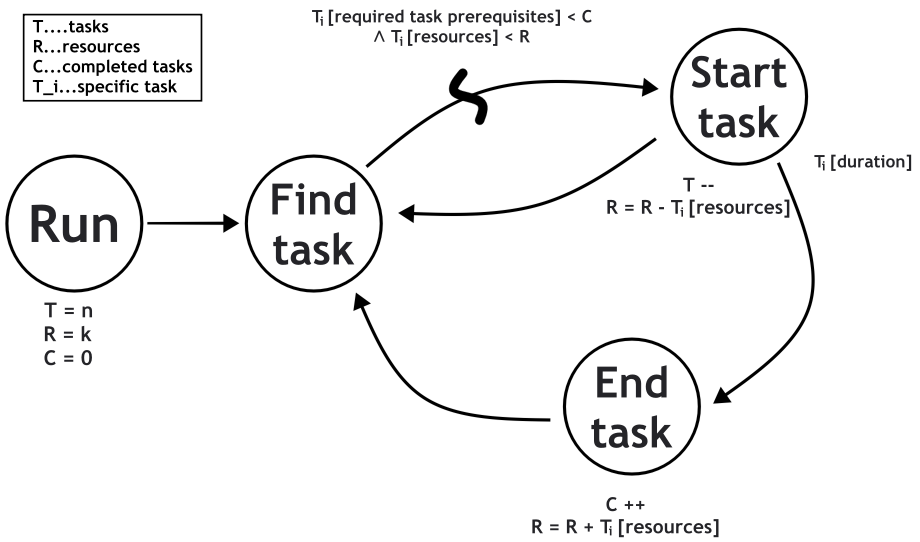
\includegraphics[scale=.4]{/Users/lanar/Documents/Cooking-model/Documentation/images/graph.png}}
    \caption{Discrete simulation graph of a cooking process.}
    \label{fig1}
\end{figure}

On this figure \ref{fig1}, we can see a simplified graph on how the simulation works. We start by calling the method \texttt{find\_task}, this as suggested searches for a task that can be executed, meaning all resources needed are available 
and all tasks, that needed to be done before, are already completed. If we find such a task, method \texttt{start\_task} is called, where the previously mentioned resources are taken of the list, the task name is added to the order and the method \texttt{schedule\_end\_task} is invoked. 
There we make an event, where we calculate the time when it will be finished by adding up duration to 'current time' and save the name of the task. This is appended to the \texttt{event\_queue} list. Directly after, the method \texttt{find\_task} is executed again. \\ 

Right at the start we start a while loop, that will be done once. The number of completed tasks is the same as the number of tasks at the start. 
With each iteration of the loop, the time increases by one. We also use this to check if there is an event scheduled at the current time. In case there is one we call the method \texttt{end\_task}. 
This is where the previously removed resources are added back to the list and the task is added to the list of completed tasks. 

At the end the function \texttt{run\_simulation} returns a tuple, where the first component is the time it took, and the second the order in which the tasks were completed. 
In case the you one does not have the required resources needed for the recipe, the program returns the error: \texttt{You do not have the right resources}.

Now that we got our program to execute a recipe, we started to work on finding the optimal ordering of tasks, to get the shortest time. 

\subsection{Different orders of tasks}
The first idea we got, was just to try all possible permutations of the list of tasks. Run the simulation for each one of them and then choose the one with the shortest time.
To help with understanding the code and making sure it worked well, we made sure to get a list of all possible orders and the time it took. Furthermore due to prior task prerequisites the recipe we had at the start returned us the same duration, no mater the order of tasks. 
To fix it we added a task, to have a three-task process, meaning heating the water, peeling potatoes and cooking them. Moreover, we changed some of the durations of tasks. 

When running the code we realized, that the order of the last few tasks rarely changes. This was caused by the prior task prerequisites, since these tasks can only be done once the others are completed.
Below you can see some of the possible orders we got. 

\begin{verbnobox}[\fontsize{8pt}{8pt}\selectfont]
[cutting meat, heating water, cutting onions, cooking meat, frying onions, cooking potatoes, cooking everything] 
[cutting meat, cutting onions, heating water, cooking meat, frying onions, cooking potatoes, cooking everything] 
[heating water, cutting meat, cutting onions, cooking meat, frying onions, cooking potatoes, cooking everything] 
[heating water, cutting onions, cutting meat, cooking meat, frying onions, cooking potatoes, cooking everything] 
[cutting onions, cutting meat, heating water, cooking meat, frying onions, cooking potatoes, cooking everything] 
[cutting onions, heating water, cutting meat, cooking meat, frying onions, cooking potatoes, cooking everything] 
\end{verbnobox}

This gave us the idea, that instead of testing all possible orders, we should firstly check which tasks are required to be done first and put those at the start of the list. 
Furthermore, the ones, who are required for more tasks, should be done first, meaning put at the start of the list, and others, which are not required for any task, should be left behind.
With this in mind we wrote the function \texttt{smart\_permutations}, which takes the name of the recipe json file and returns some permutations of the tasks, where we know one of them will give us the best order. 
Here we can see the simplified process:

\begin{verbnobox}
- get tasks from json file
- for task in all tasks:
    get task prerequisites (can be repeated)
- count repetitions of tasks
- sort in lists based on number of repetitions
- get all other tasks
- permutate each task list separately
- make all possible combinations 
\end{verbnobox}

This is afterwards inputed into the function \texttt{run}, which tries all the given orders and returns the one with the shortest duration. 


\subsection{Introducing randomness}
Since cooking does not always go as planned, we added some randomness, by prolonging/shortening the duration of tasks. 
We started by defining a parameter \texttt{time\_change\_factor} at the start of the code, which states for maximum, how many 'seconds' can a task be prolonged or shortened. 
This is all done in the function \texttt{time\_randomness} that is called when scheduling a task and calculating the time it will be completed. 
The following graph of our simulation is on figure \ref{fig2}, where the function \textit{f} represents the previously mentioned function. 

\begin{figure}[H]
    \centerline{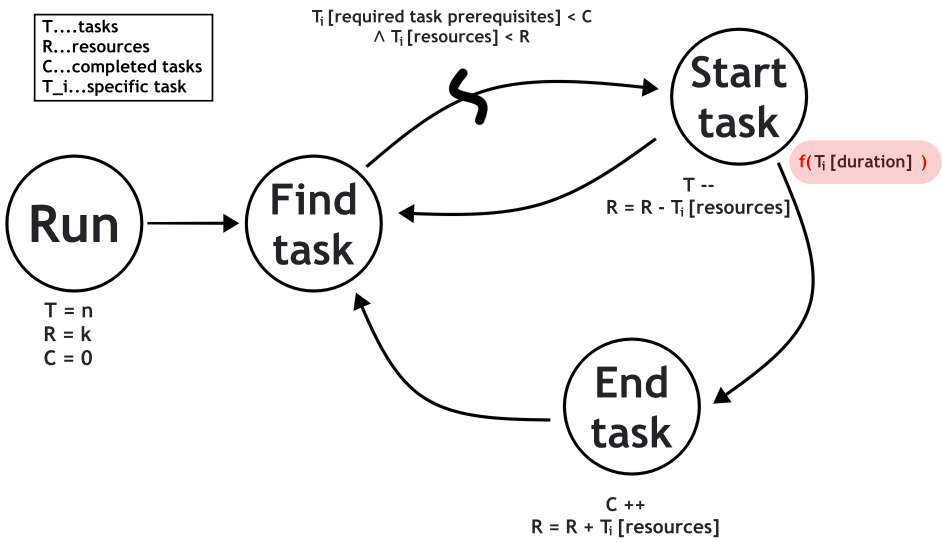
\includegraphics[scale=.23]{/Users/lanar/Documents/Cooking-model/Documentation/images/graph_showing_time.png}}
    \caption{Discrete simulation graph of a cooking process with time randomness.}
    \label{fig2}
\end{figure}




\newpage
\section{Simulation Results}
For the simulation results we looked into a few different \textcolor{red}{things}.

\subsection{Effect of different ordering}
We wanted to see how big of an impact has the order of the tasks. That is why we looked for the best order for the recipe for goulash, and the worst one. This means the one that is done the quickest and the one that takes the longest.
The following results are done with two cooks and time randomness.

\begin{verbnobox}[\fontsize{10pt}{10pt}\selectfont]
BEST ORDER: 168, 
[cutting meat, peeling potatoes, heating water, cutting onions, cooking meat, 
cooking potatoes, frying onions, cooking everything]
\end{verbnobox}

\begin{verbnobox}[\fontsize{10pt}{10pt}\selectfont]
WORST ORDER: 253,
[cutting onions, cutting meat, heating water, cooking meat,
 frying onions, peeling potatoes, cooking potatoes, cooking everything]
\end{verbnobox}

We can see that the difference in duration is 55 units of time, which is not small. 
This happens due to probalistic duration of time, but even without that, the difference would still be 30 units. The reason for that is the order of the first few tasks, 
which have to be done before cooking potatoes and cooking everything. If they are not done in the best order, the simulation has to wait for a task to be finished before doing anything new. 

\begin{figure}[H]
    \centerline{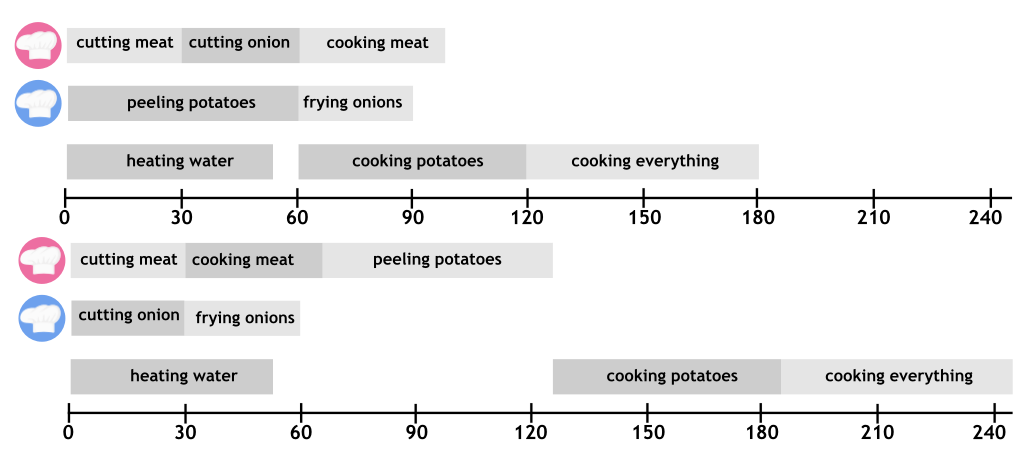
\includegraphics[scale=.4]{/Users/lanar/Documents/Cooking-model/Documentation/images/recipes_order.png}}
    \caption{The best and worst order of tasks.}
    \label{fig3}
\end{figure}

After seeing the difference an order of tasks can have, we were interested to see what are all possible durations of the recipe and which are the most common. 
In the histogram below we can make out that most of the time the recipe is completed in between 179 to 184 units of time, this suggests the order was similar to the best order as seen above, with just some different permutations of the first few tasks.

\begin{figure}[H]
    \centerline{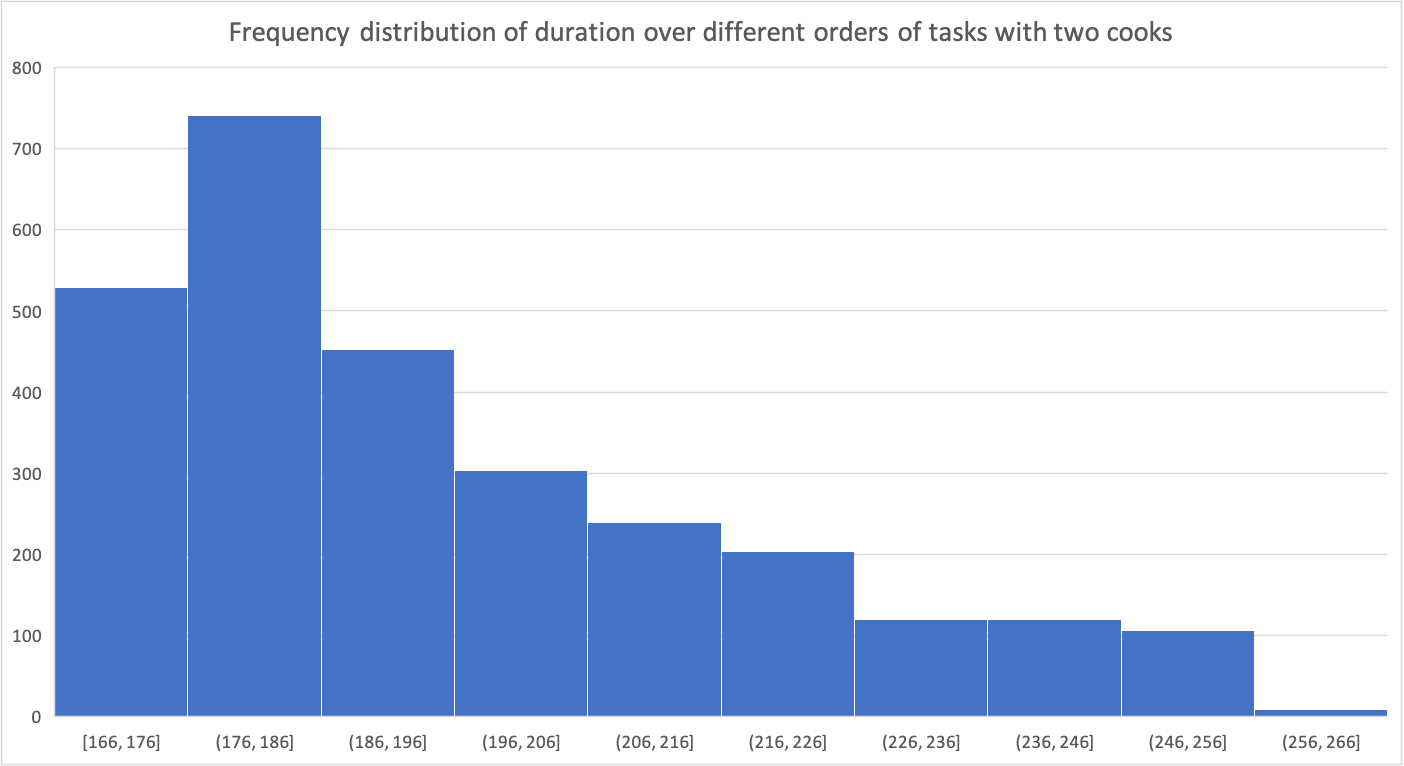
\includegraphics[scale=.5]{/Users/lanar/Documents/Cooking-model/Documentation/images/graph_duration.png}}
    \caption{All possible durations of the recipe with two cooks, devided into groups by time interval 5 units.}
    \label{fig4}
\end{figure}

We also did the same calculations for just one cook, but got a somewhat different distrubution, with most of the odrers gathered in the middle. In this case the different durations were only a result of probalistic time assignment, 
because when we ran the stohastic model, we only got one option of duration which is 251. This can be seen on the graph where most orders are between 243 to 248 units of time. 

\begin{figure}[H]
    \centerline{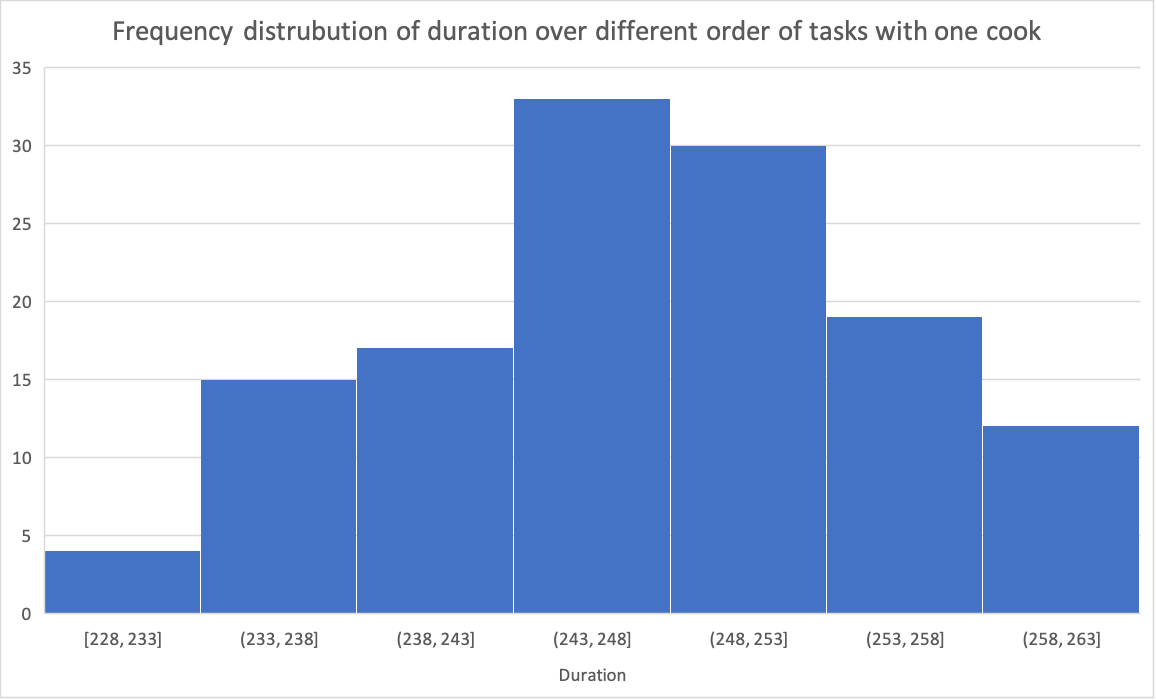
\includegraphics[scale=.5]{/Users/lanar/Documents/Cooking-model/Documentation/images/graph_duration1.png}}
    \caption{All possible durations of the recipe with one cook, devided into groups by time interval 5 units.}
    \label{fig5}
\end{figure}

\newpage
\subsection{Recipe comparison to cook book}
For our second dish we decided to do potato salad. We found a recipe in a cook book and adjusted it to our program. We wanted to test if the calculated optimal order for one cook matches the order in the cook book.
Here we can see the two orders:

\begin{verbnobox}[\fontsize{10pt}{10pt}\selectfont]
    COOK BOOK:                                  OPTIMAL ORDER:
    - cooking potatoes                          - cooking potatoes
    - cooking eggs                              - cooking eggs
    - cutting pickles                           - cutting onions
    - cooling eggs                              - make dressing
    - cutting onions                            - cutting pickles
    - peeling eggs                              - cooling eggs
    - cutting eggs                              - peeling eggs
    - peeling potatoes                          - peeling potatoes
    - cuttting potatoes                         - cutting potatoes
    - make dressing                             - cutting eggs
    - mixing enerything                         - mixing enerything
\end{verbnobox}

We can see that the two orders don not differ much. Some tasks are done in different order, but those are mainly interchangable. One different thing is when the dressing is done. 
But this is because in real life you would want it to be freshly done before completing the salad, and our program does not take this into account. 

\subsection{Different number of resources}
Lastly we focused on the number of resources to see if it really has that big of an effect on duration. 
We ran the program 5 times for each number of cooks and took the average of the optimal time. We gave the other resources a high enough quantity so that it won't effect the duration.
These are the graphs we got.

\begin{figure}[H]
    \centering
    \begin{minipage}{.5\textwidth}
      \centering
      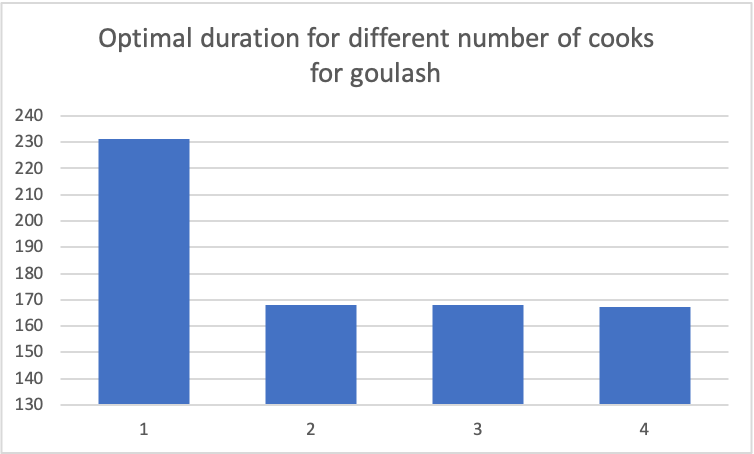
\includegraphics[width=.9\linewidth]{/Users/lanar/Documents/Cooking-model/Documentation/images/optimal_durationG.png}
      \caption{Duration of recipe goulash with \\ different number of cooks}
      \label{fig6}
    \end{minipage}%
    \begin{minipage}{.5\textwidth}
      \centering
      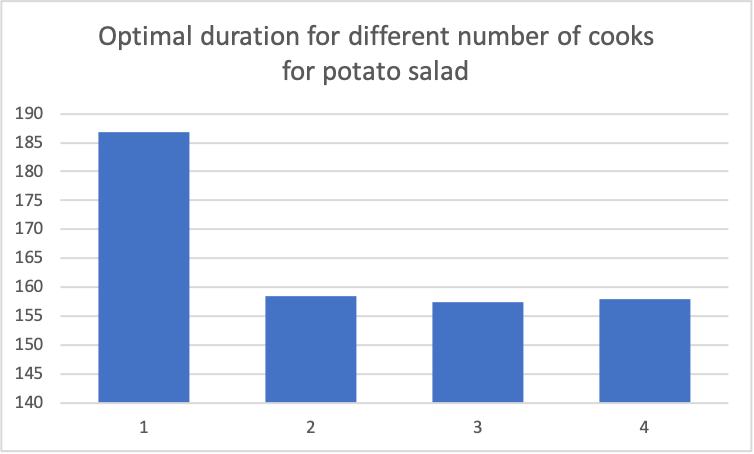
\includegraphics[width=.9\linewidth]{/Users/lanar/Documents/Cooking-model/Documentation/images/optimal_durationS.png}
      \caption{Duration of recipe potato salad with different number of cooks.}
      \label{fig7}
    \end{minipage}
\end{figure}

As you can see there is only a difference when using one or two cooks, after that you can use as many as you want, but the duration won't change. 
This is because the tasks in our recipes already have an order in which they have to be done and even if you have another cook, he still has to wait for the other task to finish. 
To test our program we decided to make another recipe, where we tried to do it so, that a different number of cooks will have a bigger effect.

\begin{figure}[H]
    \centerline{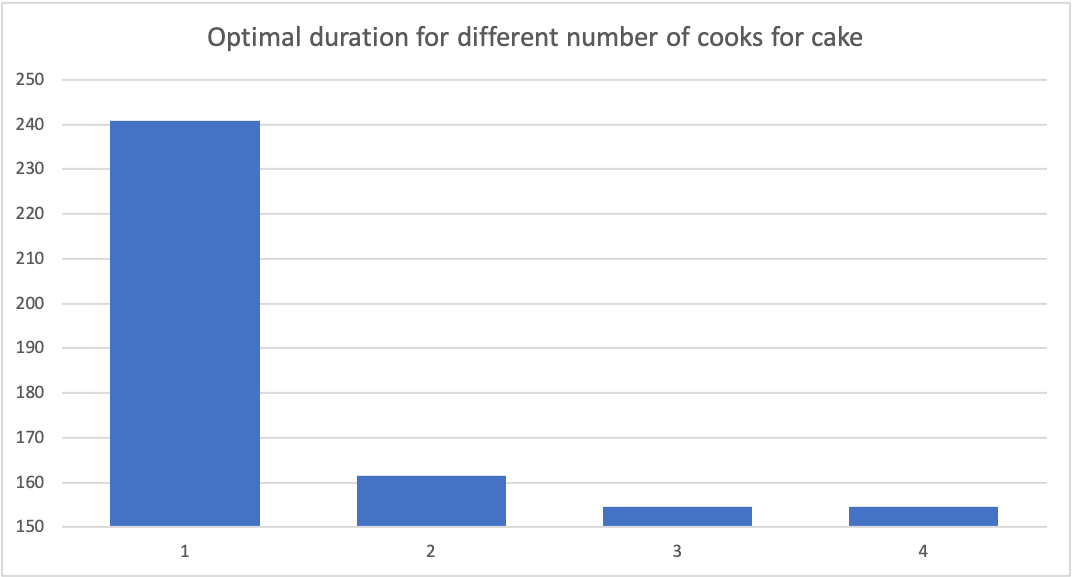
\includegraphics[scale=.5]{/Users/lanar/Documents/Cooking-model/Documentation/images/graph_durationC.png}}
    \caption{Duration of recipe cake with different number of cooks.}
    \label{fig8}
\end{figure}

These are the results we got with implementing the recipe of baking a cake. We wanted to have more independant tasks and less strict prior ordering. 
In this recipe you have to do a lot of tasks independantly and then there is just a few tasks that combine all of them. This way you can see a difference 
between one, two and three cooks, but when it comes to four, the duration still remains the same. FUrthermore the difference was very small, only 6 time uhnits. This brings us to the conslusion that with every recipe 
there will be a point where the number of cooks doesn't matter anymore. 

%ADD GRAPH FOR POTATO SALAD, ONLY ONE OF EVERY RESOURCE

Besides observing the effect of the number of cooks, we did the same for other resources. Here you can see the duration for making goulash when having:
\begin{itemize}
    \item double of everything: 181
    \item only one pan: 191
    \item only one knife: 181
\end{itemize}

This is because in the optimal recipe two knives are never used at the same time, while the pan is used for cooking the meat and frying the onions which is done at the same time. 

\begin{figure}[H]
    \centerline{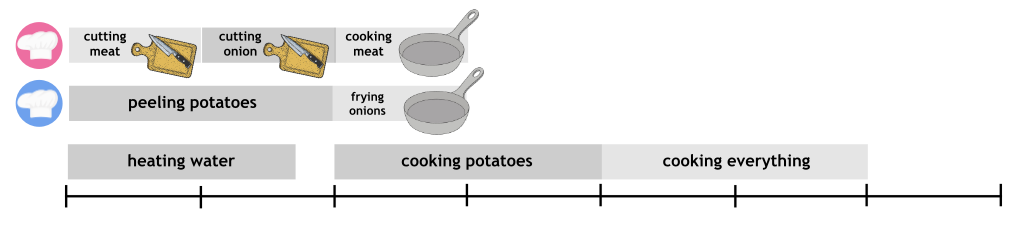
\includegraphics[scale=.4]{/Users/lanar/Documents/Cooking-model/Documentation/images/resources.png}}
    \caption{Use of pan and knife in the optimal order of the recipe goulash.}
    \label{fig9}
\end{figure}


\newpage
\section{Conclusion}
In conclusion, we breathly summarize our group work. Theme of the work was Cooking Process Simulation. We chose the program language Python. As was said before, we see some benefits in using it. also to use the json files to be the program more user friendly and also to have it more visually clear. \\

The results, that have been gotten, are describe in detail in the previous chapter. The main goal is ....\\

We conclude that We enjoyed the group work. We are familiar that our simulation program can get improved in the future. Unfortunately, there are some missing points-small mistakes. However, we hope that they have no that big impact on the running the program and the simulation in general.  


- problems code, did in simpy, turned ou to not be good \\
- three recipes, simulate the results, some especially with a cause \\
- the order does affect the time, best to do long tasks first, with more cooks there is a diffrence, with one it is almost not important \\
- got similar order, didn't take into account things like being fresh, with some tasks order not important \\
- number of cooks only important to some number, big difference between 1 and 2, resources highly effect the time, need to have more pans/knives not just cooks \\







\newpage

\bibliographystyle{plain}
\bibliography{References}

\end{document}
